\documentclass[Main]{subfiles}
\begin{document}

\chapter{Data to record}
The system must record the data described in this chapter. The user can create, view, and change the data through the tasks described in Chapter \ref{cha:C}. 
In many cases data has to be exchanged with external systems as specified in Chapter \ref{cha:F}.

Figure \ref{fig:Datamodel} is a data model that gives an overview of the data. 
Each box is a class of data. 
Imagine a pile of file cards behind the box. 
The box symbolizes one of the cards. 

There are relationships between the boxes, shown as lines.
Data need not be structured this way in the system, but it must be handled in some way. 

The data model is created using UML. The black diamond relationship (composition) refers to records of these types being directly tied together, whereas the other relations are weaker references. 

\begin{figure}[hbtp]
\centering
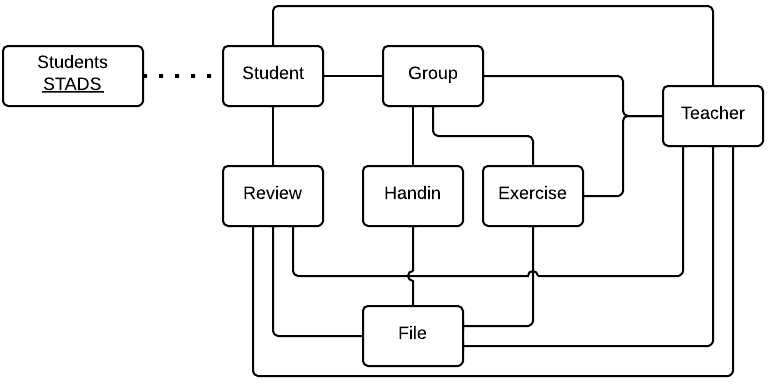
\includegraphics[width=1\textwidth]{DataModel}
\caption{Datamodel}
\label{fig:Datamodel}
\end{figure}


\newpage

\section{Student}\label{sec:DataStudent}
A \textit{Student} is a one of the participants of the course.
\begin{DataIntro}
\rSource{Students are enrolled at the start of the course. 
Students are imported from STADS.}
\rUse{Students are assigned to a \textit{Group} and can have speciel case regarding handins.}
\end{DataIntro}

\begin{DataTable}

\Record
{Student number. 
\\
Copied from the STADS database. Each student have a personal number assigned by the university to identify them. This must be shown along with a student's handin and review. }
{This can serve as a static reference.}
{}

\Record
{Full name.\\
Copied from the STADS database.
This must be shown along with a student's handin and review.}
{.}
{}

\Record
{Email address. \\
Imported from the STADS database.}
{When a notification is ready for a student it can be send to this email}
{}
\end{DataTable}


%\newpage

\section{Group}
A \textit{Group} is a list of students who will deliver handins together.
\begin{DataIntro}
%\rExample{}
\rSource{Have a minimum size of 1 student.}
\rUse{Groups deliver handins.
A group can be of only 1 student should this student choose to deliver a handin on his/her own.
Each student can only be assigned to one group pr. course.}
\end{DataIntro}

\newpage
\begin{DataTable}

\Record
{Name. \\
Autogenerated. Must be shown for the teacher on reviews.}
{}
{}


\Record
{List of students. \\
Each student of the group shall be listed here.}
{}
{}


\end{DataTable}




%\newpage

\section{Teacher}
A \textit{Teacher} is a lecturer of the course.

\begin{DataIntro}
%\rExample{}
\rSource{There will be at least 1 teacher at a course.}
\rUse{Teachers upload exercises and deadline.\\
Teachers approve reviews.}
\end{DataIntro}

\begin{DataTable}

\Record
{Initials. \\
Each teacher has initials to serve as reference for uploading exercises.}
{}
{}

\Record
{Full name.}
{Name of the teacher can be shown on exercises and notifications for students.}
{}

\Record
{Email address,}
{Email of the teacher can be shown on exercises and notifications for students.}
{}

\end{DataTable}



%\newpage

\section{Exercise}\label{sec:exercise}
An \textit{Exercise} is a a description for a task, and the students submit solutions(\textit{Handins}) in groups.
\begin{DataIntro}
%\rExample{}
\rSource{Created by a \textit{Teacher}.}
\rUse{\textit{Students} most solve the exercises within the provided deadline in groups.}
\end{DataIntro}

\newpage
\begin{DataTable}

\Record
{Name. \\
Each exercise has a name to be displayed for the students.}
{}
{}

\Record
{Deadline. \\
A date the students must deliver handins before.}
{}
{}

\Record
{Review deadline. \\
A date the students must deliver reviews before.}
{}
{}

\Record
{File(s). \\
An exercise can contain one or more files.}
{}
{}


\Record
{Commentary. \\
An exercise can have a comment on it.}
{}
{}


\Record
{Timestamp. \\
A date for when uploaded.}
{}
{}
\end{DataTable}




%\newpage

\section{Handin}

	
\begin{DataIntro}
%\rExample{}
\rSource{Student upload handins.}
\rUse{Handins will be assigned to review for other students.}
\end{DataIntro}

\begin{DataTable}

\Record
{Group name, \\
Name for the group who delivered it.}
{}
{}

\Record
{File(s). \\
An exercise can contain one or more files.}
{}
{}


\Record
{Commentary. \\
An exercise can have a comment on it.}
{}
{}


\Record
{Timestamp.}
{A date for when uploaded.}
{}
\end{DataTable}






\newpage

\section{Review}
Reviews are made by a single student for another student's handin. 
The review can be uploaded multiple time in different versions -- only the last will be shown to the other student.

\begin{DataIntro}
%\rExample{}
\rSource{Student.}
\rUse{The reviews include notes for improvement for the other student.}
\end{DataIntro}

\begin{DataTable}


\Record
{Student ID. \\
Reviewer's student ID to trace who reviews the handin.}
{}
{}


\Record
{Timestamp. \\
Used to track when the review has been uploaded.}
{}
{}


\Record
{File(s). \\
Optional -- contains comments for the handin.}
{}
{}


\Record
{Comments.\\
Optional if no file has been uploaded -- contains comment for the handin.}
{}
{}

\Record
{Overall assessment. \\
A yes/no indication of the review result.}
{}
{}

\Record
{Ready for deliver.\\
Field must be checked to deliver a review, should one change mind after a review.
This must be checked before the deadline.}
{}
{}
\end{DataTable}




%\newpage

%\section{Files}
%Files will be multiple versions of exercises, handins and reviews.
%All versions must be saved and possible to retrieve.
%
%\begin{DataIntro}
%\rExample{}
%\rSource{Uploads as exercises, handins or reviews.}
%\rUse{These files can be downloaded and uploaded by students for when submitting handins, when viewing an exercise, submitting reviews and looking at reviews of own handins.}
%\end{DataIntro}
%
%\begin{DataTable}
%
%\Record
%{ID}
%{Unique identifier for system retrieval and storage.}
%{}
%
%
%\Record
%{Name}
%{The name of the file}
%{}
%
%
%\Record
%{Binary storage}
%{Storage of the file can be done in binary form}
%{}
%\end{DataTable}





\end{document}
